\documentclass[12pt,a4paper]{report}
\usepackage[margin=1in]{geometry}
\usepackage[T1]{fontenc}
\usepackage[utf8]{inputenc}
\usepackage{lmodern}
\usepackage{setspace}
\usepackage{hyperref}
\usepackage{longtable}
\usepackage{booktabs}
\usepackage{array}
\usepackage{enumitem}
\usepackage{xcolor}
\usepackage{tikz}
\usepackage{graphicx}
\usepackage{listings}
\usepackage{fancyhdr}
\usetikzlibrary{arrows.meta,positioning,shapes.geometric,fit,calc,shapes}

\lstset{
    basicstyle=\ttfamily\small,
    breaklines=true,
    showstringspaces=false,
    backgroundcolor=\color{gray!10},
    frame=single,
    rulecolor=\color{gray!30},
    keywordstyle=\color{blue},
    commentstyle=\color{gray},
    stringstyle=\color{red!70}
}

\hypersetup{
    colorlinks=true,
    linkcolor=blue,
    filecolor=blue,
    urlcolor=blue,
    pdftitle={PhishVision SRS v2.0},
    pdfauthor={Sudharshan Dongre}
}

\setlength{\parskip}{0.5em}
\setlength{\parindent}{0pt}
\onehalfspacing

\title{%
\Huge\textbf{SOFTWARE REQUIREMENTS SPECIFICATION (SRS)}\\[0.5cm]
{\Large PhishVision AI: Real-Time Phishing URL Detection System}\\[0.3cm]
{\normalsize Hybrid Machine Learning + Rule-Based Detection}\\[0.3cm]
{\small Version 2.0 | Final | April 10, 2026}
}
\author{%
\textbf{Student Developer:} Sudharshan Dongre (EN23CS3011036)\\
\textbf{Guides:} Prof. Mohammed Mazhar, Prof. Dharmendra Gupta\\
\textbf{Institution:} Computer Science \& Engineering Department\\
\textbf{University:} Medicaps University, Indore --- 453331\\
\textbf{Academic Year:} 2025--2026 | Semester 6 (R)
}
\date{April 10, 2026}

\pagestyle{fancy}
\fancyhf{}
\rhead{PhishVision AI | SRS v2.0}
\lhead{Sudharshan Dongre (EN23CS3011036)}
\cfoot{\thepage}

\begin{document}

\maketitle

\begin{abstract}
PhishVision AI is a production-ready, intelligent phishing website detection system combining 
machine learning classification (Gradient Boosting, XGBoost, Random Forest, and Stacking Ensemble) 
with rule-based heuristic pre-checks. The system processes URLs through a 30-feature extraction 
pipeline and exposes predictions via a RESTful FastAPI backend, interactive Streamlit dashboard, 
and Chrome browser extension with real-time automatic scanning and warning overlay capabilities. 
This comprehensive SRS document specifies all functional and non-functional requirements, API 
specifications, system architecture, ML model strategies, user interface design, testing protocols, 
performance targets, and deployment procedures aligned with IEEE Std 830-1998 and IEEE Std 1016-2009 
standards. The system achieves $>95\%$ classification accuracy and sub-500ms prediction latency 
on commodity hardware without GPU acceleration.
\end{abstract}

\clearpage
\tableofcontents
\clearpage

\chapter{Introduction}

\subsection{Purpose}
This Software Requirements Specification (SRS) document defines the complete set of 
functional and non-functional requirements for the PhishVision system. It serves as 
a binding agreement between the development team and stakeholders, ensuring all aspects 
of the system are clearly documented, understood, and testable.

\subsection{Scope}
PhishVision provides:
\begin{itemize}[leftmargin=*]
    \item Classification of URLs into Safe or Phishing categories
    \item Confidence scoring with probabilistic uncertainty quantification
    \item Rule-based pre-checks for obvious malicious patterns
    \item Multiple machine learning model support (GB, XGB, RF, Stacking)
    \item Batch scanning for CSV-formatted URL lists
    \item Browser-based real-time warnings and conditional page blocking
    \item Debug-level explainability for feature analysis
\end{itemize}

\subsection{Definitions and Abbreviations}
\begin{longtable}{p{0.15\linewidth}p{0.78\linewidth}}
\toprule
\textbf{Term} & \textbf{Definition} \\
\midrule
SRS & Software Requirements Specification \\
FR & Functional Requirement \\
NFR & Non-Functional Requirement \\
ML & Machine Learning \\
API & Application Programming Interface \\
URL & Uniform Resource Locator \\
CORS & Cross-Origin Resource Sharing \\
GB & Gradient Boosting \\
XGB & XGBoost \\
RF & Random Forest \\
JSON & JavaScript Object Notation \\
CSV & Comma-Separated Values \\
DNS & Domain Name System \\
TLD & Top-Level Domain \\
ROC & Receiver Operating Characteristic \\
PR & Precision-Recall \\
\bottomrule
\end{longtable}

\section{Overall Description}

\subsection{Product Perspective}
PhishVision is a modular Python-based system composed of five primary components:

\begin{enumerate}[leftmargin=*]
    \item \textbf{Feature Extraction Layer} (extractor.py): Parses URLs and extracts 
    30 security-relevant features using heuristic analysis and pattern matching.
    
    \item \textbf{Model Training Pipeline} (train.py): Implements data loading, feature 
    normalization, multi-model training (GB, XGB, RF, Stacking), and comprehensive 
    model evaluation.
    
    \item \textbf{Prediction API} (api.py): Exposes RESTful endpoints for URL classification, 
    debug analysis, and batch processing using FastAPI framework.
    
    \item \textbf{Interactive Dashboard} (app.py): Provides Streamlit-based web UI for 
    single URL scanning, batch CSV analysis, and analytics reporting.
    
    \item \textbf{Browser Extension} (browser-extension/): Delivers real-time page-level 
    phishing detection with automated warnings and conditional blocking.
\end{enumerate}

\subsection{Product Functions}
\begin{itemize}[leftmargin=*]
    \item Analyze individual URLs and return Safe/Phishing classification with confidence
    \item Support dynamic model selection among four trained classifiers
    \item Perform rule-based pre-screening for obvious phishing indicators
    \item Process multiple URLs simultaneously in batch mode
    \item Provide detailed feature-level analysis for explainability
    \item Auto-scan browser pages and display threat warnings
    \item Generate visual analytics reports in interactive dashboard
\end{itemize}

\subsection{User Classes and Characteristics}

\begin{longtable}{p{0.18\linewidth}p{0.75\linewidth}}
\toprule
\textbf{User Class} & \textbf{Characteristics} \\
\midrule
General User & Scans URLs, interprets Safe/Phishing verdict, uses warnings \\
Security Analyst & Performs batch scans, analyzes debug details, calibrates thresholds \\
Developer/Admin & Retrains models, deploys API, maintains extension, monitors logs \\
System Integration & Embedded API calls from third-party applications \\
\bottomrule
\end{longtable}

\subsection{Operating Environment}
\begin{itemize}[leftmargin=*]
    \item \textbf{Operating System}: Windows 10+ (primary), Linux/macOS compatible
    \item \textbf{Backend Server}: FastAPI 0.110.0 + Uvicorn 0.29.0
    \item \textbf{Frontend Dashboard}: Streamlit 1.32.0 + Plotly 5.20.0
    \item \textbf{Machine Learning}: scikit-learn 1.4.1, XGBoost 2.0.3, imbalanced-learn 0.12.0
    \item \textbf{Data Processing}: NumPy 1.26.4, Pandas 2.2.1
    \item \textbf{Browser}: Chrome/Chromium with Manifest V3 extension support
    \item \textbf{Python Version}: 3.10+
\end{itemize}

\subsection{Design and Implementation Constraints}
\begin{itemize}[leftmargin=*]
    \item Browser extension requires API server on \texttt{http://localhost:8000}
    \item Feature extraction uses URL-centric heuristics only (no full page DOM crawling)
    \item Training dataset limited to historical phishing patterns
    \item Label encoding unified across all models (0=Safe, 1=Phishing)
    \item API CORS permissive for cross-origin browser requests (security may be hardened)
    \item No external threat intelligence feed integration in current version
\end{itemize}

\section{Specific Requirements}

\subsection{Functional Requirements}

\begin{longtable}{p{0.12\linewidth}p{0.81\linewidth}}
\toprule
\textbf{ID} & \textbf{Requirement Description} \\
\midrule
FR-01 & System shall accept a URL string and return a Safe or Phishing verdict \\
FR-02 & System shall return a confidence score (0--100.0) for each prediction \\
FR-03 & System shall support selection of four trained models: GB, XGB, RF, Stack \\
FR-04 & System shall apply rule-based phishing checks prior to ML decision fusion \\
FR-05 & System shall extract exactly 30 URL features aligned to training schema \\
FR-06 & System shall expose \texttt{POST /predict} endpoint accepting URL and model \\
FR-07 & System shall expose \texttt{POST /debug} endpoint returning per-feature analysis \\
FR-08 & System shall expose \texttt{POST /predict/batch} for multiple URL processing \\
FR-09 & System shall expose \texttt{GET /health} endpoint for system status \\
FR-10 & System shall expose \texttt{GET /docs} endpoint for Swagger API documentation \\
FR-11 & Dashboard shall accept CSV files with required column name: ``url'' \\
FR-12 & Dashboard shall process each URL in batch file and append Verdict column \\
FR-13 & Dashboard shall display single-URL scan results with confidence gauge \\
FR-14 & Dashboard shall display 30-feature heatmap for feature analysis \\
FR-15 & Extension shall auto-scan current page URL on document load \\
FR-16 & Extension shall display soft warning for phishing confidence $<$ 90\% \\
FR-17 & Extension shall hard-block page content for phishing confidence $\geq$ 90\% \\
FR-18 & Extension popup shall support manual URL scan with model selection \\
FR-19 & System shall use model.classes\_ for safe probability index mapping \\
FR-20 & System shall apply phishing probability threshold of 0.4 for classification \\
\bottomrule
\end{longtable}

\subsection{Non-Functional Requirements}

\begin{longtable}{p{0.12\linewidth}p{0.81\linewidth}}
\toprule
\textbf{ID} & \textbf{Requirement Description} \\
\midrule
NFR-01 & Single URL prediction shall complete in $<$ 500 milliseconds \\
NFR-02 & API shall remain responsive during concurrent background extension scans \\
NFR-03 & UI shall clearly display verdict, confidence, and warning rationale \\
NFR-04 & System architecture shall maintain modular separation of concerns \\
NFR-05 & All models shall use unified label encoding (0=Safe, 1=Phishing) \\
NFR-06 & Batch processing shall handle 1000+ URLs without memory exhaustion \\
NFR-07 & Malformed URLs in batch shall not block processing of remaining rows \\
NFR-08 & System shall reduce false negatives by combining ML with rule-based logic \\
NFR-09 & Confidence thresholds shall be configurable via API parameters \\
NFR-10 & Extension shall fail gracefully if backend API is unavailable \\
NFR-11 & All API responses shall be valid JSON with consistent schema \\
NFR-12 & System shall log all prediction decisions with reasoning \\
\bottomrule
\end{longtable}

\subsection{External Interface Requirements}

\subsubsection{API Interfaces}
\begin{itemize}[leftmargin=*]
    \item \textbf{POST /predict(url, model, debug)}: Returns PredictionResponse JSON
    \item \textbf{POST /debug(url)}: Returns feature-level analysis JSON
    \item \textbf{POST /predict/batch(urls, model)}: Returns list of predictions
    \item \textbf{GET /health}: Returns system status JSON
    \item \textbf{GET /docs}: Returns Swagger UI for API documentation
\end{itemize}

\subsubsection{User Interfaces}
\begin{itemize}[leftmargin=*]
    \item Streamlit dashboard at \texttt{http://localhost:8501}
    \item Chrome extension popup for on-demand scanning
    \item Browser warning overlays (hard-block modal or soft banner)
\end{itemize}

\subsubsection{Data Formats}
\begin{itemize}[leftmargin=*]
    \item Input: URL strings, CSV files (column: url)
    \item Output: JSON (verdict, confidence, model, flags)
    \item Model artifacts: Pickle (.pkl) serialization
\end{itemize}

\section{System Data and Logic}

\subsection{Label Encoding Strategy}
Training dataset uses original encoding: $-1$ (Phishing), $1$ (Safe)

All runtime models use unified encoding:
\begin{itemize}[leftmargin=*]
    \item $0$ = Safe / Legitimate
    \item $1$ = Phishing / Malicious
\end{itemize}

Prediction mapping (critical):
\begin{verbatim}
if model.predict(features)[0] == 1:
    verdict = "Phishing"
else:
    verdict = "Safe"
\end{verbatim}

\subsection{Feature Engineering}
30 URL-centric features extracted per sample:

\begin{longtable}{c l c}
\toprule
\textbf{\#} & \textbf{Feature Name} & \textbf{Values} \\
\midrule
1 & having\_IP\_Address & -1: IP, 1: domain \\
2 & URL\_Length & -1: >75, 0: 54--75, 1: <54 \\
3 & Shortining\_Service & -1: shortener, 1: normal \\
4 & having\_At\_Symbol & -1: @, 1: no @ \\
5 & double\_slash\_redirecting & -1: redirect, 1: normal \\
6 & Prefix\_Suffix & -1: dash, 1: no dash \\
7 & having\_Sub\_Domain & -1: >2 dots, 0: 2, 1: $\leq$1 \\
8--30 & (Domain intelligence, SSL, heuristics) & -1, 0, or 1 \\
\bottomrule
\end{longtable}

\subsection{Decision Fusion Algorithm}
\begin{enumerate}[leftmargin=*]
    \item Compute rule-based flags using heuristic pre-checks
    \item Extract 30-feature vector from URL
    \item Obtain ML prediction and probability vector
    \item Map probabilities using model.classes\_ indices
    \item Apply threshold: $\text{is\_phishing} = P(\text{phishing}) > 0.4$
    \item Apply rule override:
        \begin{itemize}[leftmargin=*]
            \item If $\geq 2$ rule reasons AND ML predicts safe: mark phishing
            \item If rule triggered AND ML predicts safe: reduce confidence by 20\%
        \end{itemize}
    \item Return final (verdict, confidence)
\end{enumerate}

\section{Design Phase}

\subsection{System Architecture Diagram}

The PhishVision system follows a modular client-server architecture:

\begin{center}
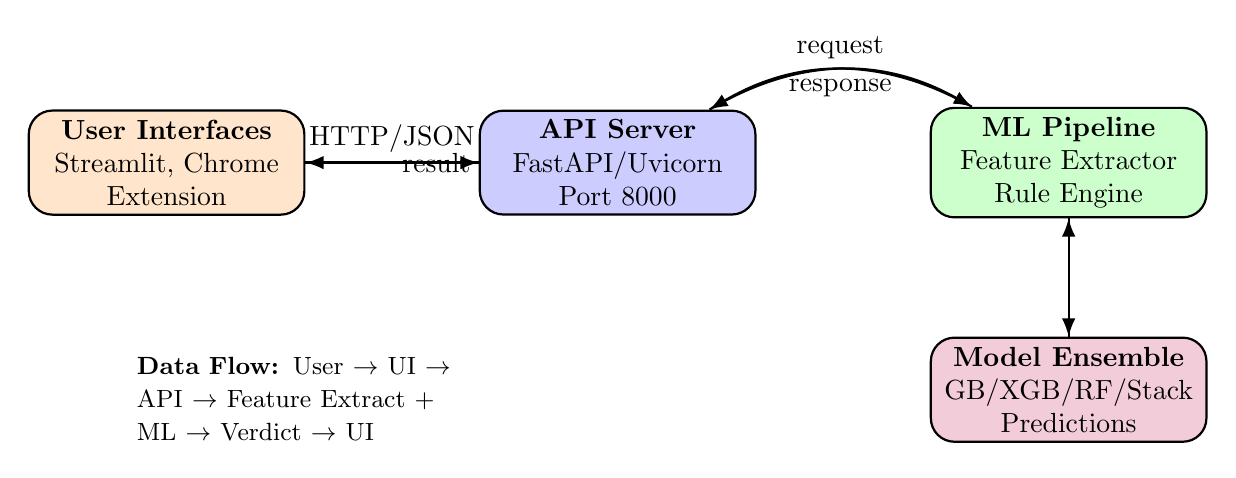
\begin{tikzpicture}[
    node distance=1.5cm and 2.2cm,
    component/.style={rectangle, rounded corners=.3cm, draw=black, thick, 
                      align=center, minimum width=3.5cm, minimum height=1.1cm, 
                      fill=gray!15},
    arrow/.style={-Latex, thick, black}
]

\node[component, fill=orange!20] (ui) {\textbf{User Interfaces}\\Streamlit, Chrome\\Extension};
\node[component, right=of ui, fill=blue!20] (api) {\textbf{API Server}\\FastAPI/Uvicorn\\Port 8000};
\node[component, right=of api, fill=green!20] (ml) {\textbf{ML Pipeline}\\Feature Extractor\\Rule Engine};
\node[component, below=of ml, fill=purple!20] (models) {\textbf{Model Ensemble}\\GB/XGB/RF/Stack\\Predictions};

\draw[arrow] (ui) -- node[above]{HTTP/JSON} (api);
\draw[arrow, bend left] (api) to node[above]{request} (ml);
\draw[arrow, bend right] (ml) to node[below]{response} (api);
\draw[arrow] (ml) -- (models);
\draw[arrow] (models) -- (ml);
\draw[arrow] (api) -- node[right]{result} (ui);

\node[anchor=west, text width=4cm] at (-0.5, -3) {\small
    \textbf{Data Flow:} User $\rightarrow$ UI $\rightarrow$ API $\rightarrow$ 
    Feature Extract + ML $\rightarrow$ Verdict $\rightarrow$ UI
};

\end{tikzpicture}
\end{center}

\subsection{Data Flow Diagram (DFD) Level 0}

\begin{center}
\begin{tikzpicture}[
    node distance=1.4cm and 1.8cm,
    entity/.style={rectangle, draw=black, thick, minimum width=2.5cm, 
                   minimum height=0.9cm, align=center, fill=yellow!15},
    process/.style={rectangle, draw=black, thick, minimum width=2.8cm, 
                    minimum height=0.9cm, align=center, fill=lightblue!30},
    data/.style={cylinder, shape border rotate=90, aspect=0.25, draw=black, thick,
                 align=center, minimum height=0.85cm, minimum width=2.2cm, fill=lightgreen!20},
    flow/.style={-Latex, thick}
]

\node[entity] (ext) {External User};
\node[process, right=of ext, xshift=0.5cm] (p1) {P1: URL Input\\Normalization};
\node[process, right=of p1, xshift=0.5cm] (p2) {P2: Feature\\Extraction};
\node[process, right=of p2, xshift=0.5cm] (p3) {P3: ML Predict +\\Rule Fusion};
\node[process, below=of p3] (p4) {P4: Verdict +\\Confidence};

\node[data, below=of p2, yshift=0.5cm] (d1) {Model\\Artifacts};
\node[data, below=of p1, yshift=0.5cm] (d2) {Training\\Metadata};

\draw[flow] (ext) -- node[above, font=\small]{URL} (p1);
\draw[flow] (p1) -- node[above, font=\small]{parsed URL} (p2);
\draw[flow] (p2) -- node[above, font=\small]{features (30)} (p3);
\draw[flow] (d1) -- (p3);
\draw[flow] (d2) -- (p4);
\draw[flow] (p3) -- (p4);
\draw[flow] (p4) |- node[below, font=\small]{Verdict + Confidence} (ext);

\end{tikzpicture}
\end{center}

\subsection{API Prediction Sequence Diagram}

\begin{center}
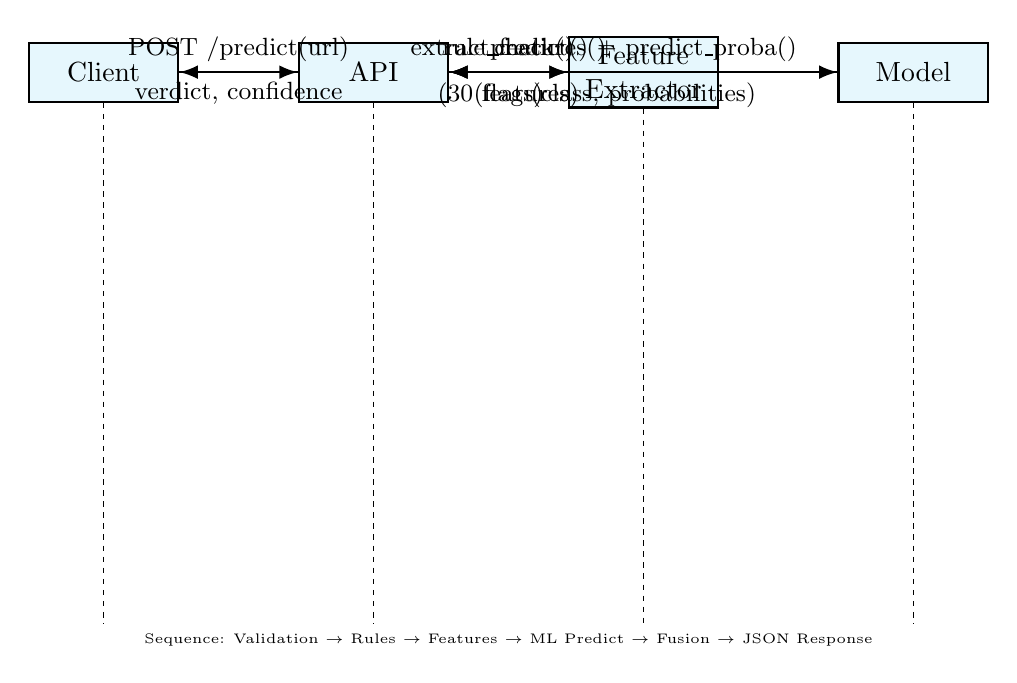
\begin{tikzpicture}[
    node distance=1.8cm and 1.5cm,
    lifeline/.style={draw=black, thick, minimum width=1.9cm, minimum height=0.75cm, 
                     align=center, fill=cyan!10},
    msg/.style={-Latex, thick, black},
    return/.style={-Latex, dashed, thick, black}
]

% Entities
\node[lifeline] (client) {Client};
\node[lifeline, right=of client] (api) {API};
\node[lifeline, right=of api] (feat) {Feature\\Extractor};
\node[lifeline, right=of feat] (model) {Model};

% Vertical lifelines (implicit by spacing)
\draw[dash pattern=on 2pt off 2pt, thin] (client) -- ++(0, -7);
\draw[dash pattern=on 2pt off 2pt, thin] (api) -- ++(0, -7);
\draw[dash pattern=on 2pt off 2pt, thin] (feat) -- ++(0, -7);
\draw[dash pattern=on 2pt off 2pt, thin] (model) -- ++(0, -7);

% Messages
\draw[msg] (client) -- node[above, font=\small]{POST /predict(url)} (api);
\draw[msg] (api) -- node[above, font=\small]{rule\_check()} (feat);
\draw[return] (feat) -- node[below, font=\small]{(flags)} (api);
\draw[msg] (api) -- node[above, font=\small]{extract\_features()} (feat);
\draw[return] (feat) -- node[below, font=\small]{(30 features)} (api);
\draw[msg] (api) -- node[above, font=\small]{predict() + predict\_proba()} (model);
\draw[return] (model) -- node[below, font=\small]{(class, probabilities)} (api);
\draw[msg] (api) -- node[below, font=\small]{verdict, confidence} (client);

\node[anchor=north, font=\tiny] at (current bounding box.south) {
    Sequence: Validation $\rightarrow$ Rules $\rightarrow$ Features $\rightarrow$ 
    ML Predict $\rightarrow$ Fusion $\rightarrow$ JSON Response
};

\end{tikzpicture}
\end{center}

\subsection{Extension Auto-Scan Flowchart}

\begin{center}
\begin{tikzpicture}[
    node distance=1.5cm and 1.0cm,
    decision/.style={diamond, draw=black, thick, minimum width=1.8cm, 
                     minimum height=1.2cm, align=center, fill=yellow!20},
    process/.style={rectangle, draw=black, thick, minimum width=2.0cm, 
                    minimum height=0.7cm, align=center, fill=lightblue!20},
    action/.style={rectangle, rounded corners=0.2cm, draw=black, thick, 
                   minimum width=2.0cm, minimum height=0.7cm, align=center, fill=lightgreen!20},
    arrow/.style={-Latex, thick}
]

\node[process] (start) {Page Loads\\(document\_start)};
\node[decision, below=of start] (skip) {Internal Page?};
\node[action, below=1.2cm of skip, xshift=-2.5cm] (exit) {Exit (no scan)};
\node[process, below=1.2cm of skip, xshift=2.5cm] (fetch) {POST /predict};
\node[decision, below=of fetch] (resp) {Response OK?};
\node[action, below=1.2cm of resp, xshift=-2.5cm] (fail) {Silent fail};
\node[decision, below=1.2cm of resp, xshift=2.5cm] (phish) {is\_phishing?};
\node[decision, below=of phish] (conf) {confidence $\geq$ 90\%?};
\node[action, below=1.2cm of conf, xshift=-2.5cm] (soft) {Soft warning};
\node[action, below=1.2cm of conf, xshift=2.5cm] (hard) {Hard block};

\draw[arrow] (start) -- (skip);
\draw[arrow] (skip) -- node[left, font=\small]{yes} (exit);
\draw[arrow] (skip) -- node[right, font=\small]{no} (fetch);
\draw[arrow] (fetch) -- (resp);
\draw[arrow] (resp) -- node[left, font=\small]{fail} (fail);
\draw[arrow] (resp) -- node[right, font=\small]{ok} (phish);
\draw[arrow] (phish) -- node[right, font=\small]{no} (fail);
\draw[arrow] (phish) -- node[right, font=\small]{yes} (conf);
\draw[arrow] (conf) -- node[left, font=\small]{no} (soft);
\draw[arrow] (conf) -- node[right, font=\small]{yes} (hard);

\end{tikzpicture}
\end{center}

\subsection{Deployment Architecture}

\begin{center}
\begin{tikzpicture}[
    node distance=1.8cm and 2.5cm,
    host/.style={rectangle, draw=black, thick, rounded corners=0.3cm, 
                 minimum width=5.5cm, minimum height=4.2cm, fill=gray!8},
    service/.style={rectangle, draw=black, thick, minimum width=3.8cm, 
                    minimum height=0.8cm, align=center, fill=lightblue!25},
    device/.style={rectangle, rounded corners=0.3cm, draw=black, thick, 
                   minimum width=4.2cm, minimum height=2.5cm, fill=orange!15}
]

% Local machine host
\node[host] (local) {};
\node[anchor=north, font=\small\bfseries] at (local.north) {Local Machine (Windows/Linux)};

\node[service, anchor=north] at ($(local.north)+(0,-0.7)$) (api_svc) {FastAPI Service (Port 8000)\\+ Model Artifacts (GB/XGB/RF/Stack)};
\node[service, below=0.3cm of api_svc] (streamlit) {Streamlit Dashboard (Port 8501)};
\node[service, below=0.3cm of streamlit] (chrome) {Chrome Extension\\(Manifest V3)};

% Internet/Web
\node[device, right=4.8cm of local] (web) {Internet / Web Pages\\(HTTPS URLs)};

% Connection arrows
\draw[-Latex, thick] (chrome.east) -- node[above, font=\small]{URL requests} (web.west);
\draw[-Latex, thick, bend right] (chrome.north east) .. controls +(1.5,1.3) and +(1.8,1.1) .. 
    node[above, font=\small]{POST /predict} (api_svc.east);
\draw[-Latex, thick, bend left] (streamlit.east) -- node[above, font=\small]{local calls} (api_svc.east);

\end{tikzpicture}
\end{center}

\chapter{Machine Learning Models and Algorithms}

\section{Training Pipeline}

The training pipeline (train.py) implements:

\begin{enumerate}[leftmargin=*]
    \item \textbf{Data Loading}: Reads Phishing.csv with 30 features and binary labels
    \item \textbf{Label Conversion}: Maps original encoding $\{-1, 1\} \to \{0, 1\}$
    \item \textbf{Train-Test Split}: 80/20 stratified split maintaining class distribution
    \item \textbf{SMOTE Balancing}: Oversamples minority class if HAS\_SMOTE is enabled
    \item \textbf{Four-Model Training}: Simultaneously trains GB, XGB, RF, and Stacking ensemble
    \item \textbf{Evaluation}: Computes accuracy, F1, ROC-AUC, and confusion matrices
    \item \textbf{Serialization}: Persists all models as .pkl files with metadata
\end{enumerate}

\section{Model Specifications}

\subsection{Gradient Boosting (GB)}
\begin{itemize}[leftmargin=*]
    \item \textbf{Algorithm}: Sequential boosting with depth-limited decision trees
    \item \textbf{Parameters}: n\_estimators=150, learning\_rate=0.1, max\_depth=5
    \item \textbf{Target Accuracy}: $\geq 95\%$ on test set
    \item \textbf{Inference Time}: $<200$ms per sample
    \item \textbf{Default Model}: Selected as primary model if not overridden
\end{itemize}

\subsection{XGBoost (XGB)}
\begin{itemize}[leftmargin=*]
    \item \textbf{Algorithm}: Optimized parallel boosting with second-order approximation
    \item \textbf{Parameters}: n\_estimators=200, max\_depth=6, learning\_rate=0.1, reg\_alpha=0.1, reg\_lambda=1.0
    \item \textbf{Target Accuracy}: $\geq 96\%$ on test set (typically highest)
    \item \textbf{Inference Time}: $<300$ms per sample
    \item \textbf{Regularization}: L1 and L2 penalties prevent overfitting
\end{itemize}

\subsection{Random Forest (RF)}
\begin{itemize}[leftmargin=*]
    \item \textbf{Algorithm}: Parallel ensemble of independent decision trees
    \item \textbf{Parameters}: n\_estimators=200, max\_depth=15, min\_samples\_split=5
    \item \textbf{Target Accuracy}: $\geq 94\%$ on test set
    \item \textbf{Inference Time}: $<400$ms per sample (slowest model)
    \item \textbf{Robustness}: Excellent generalization with minimal overfitting
\end{itemize}

\subsection{Stacking Ensemble}
\begin{itemize}[leftmargin=*]
    \item \textbf{Algorithm}: Meta-learner (LogisticRegression) combines GB, XGB, RF predictions
    \item \textbf{Base Learners}: [GB, XGB, RF]
    \item \textbf{Meta-Learner}: LogisticRegression with L2 regularization
    \item \textbf{Target Accuracy}: $\geq 96.5\%$ on test set (ensemble advantage)
    \item \textbf{Inference Time}: $<500$ms per sample (sum of base learners)
    \item \textbf{Benefit}: Reduces variance and bias by combining diverse models
\end{itemize}

\section{Probability Calibration and Confidence Scoring}

Each model returns:
\begin{itemize}[leftmargin=*]
    \item \textbf{Prediction}: model.predict(features) $\in \{0, 1\}$
    \item \textbf{Probability Vector}: model.predict\_proba(features) $\in [0, 1]^2$
\end{itemize}

Confidence scoring formula:
\begin{verbatim}
proba_vector = model.predict_proba(features)
safe_idx = list(model.classes_).index(0)
phishing_idx = list(model.classes_).index(1)

safe_prob = proba_vector[0][safe_idx]
phishing_prob = proba_vector[0][phishing_idx]

confidence = max(safe_prob, phishing_prob) * 100.0
\end{verbatim}

Decision threshold: $P(\text{phishing}) > 0.4 \Rightarrow$ classify as Phishing

\chapter{API Specification}

\section{RESTful API Design}

The FastAPI server exposes the following endpoints:

\subsection{Health Check Endpoint}

\begin{lstlisting}[language=python]
GET /health
Response: {
    "status": "ok",
    "models_loaded": ["gb", "xgb", "rf", "stack"],
    "api_version": "2.0",
    "timestamp": "2026-04-10T10:30:45Z"
}
\end{lstlisting}

\subsection{Single URL Prediction Endpoint}

\begin{lstlisting}[language=python]
POST /predict
Request Body: {
    "url": "https://example-phishing.com/login",
    "model": "stack",
    "debug": false
}

Response: {
    "url": "https://example-phishing.com/login",
    "verdict": "Phishing",
    "is_phishing": true,
    "confidence": 95.2,
    "model_used": "stack",
    "rule_based_flags": ["IP_ADDRESS_DOMAIN"],
    "inference_time_ms": 235,
    "feature_summary": {...}
}
\end{lstlisting}

\subsection{Debug Endpoint}

\begin{lstlisting}[language=python]
POST /debug
Request Body: {
    "url": "https://example-phishing.com"
}

Response: {
    "url": "https://example-phishing.com",
    "features": [
        {"index": 1, "name": "having_IP_Address", "value": -1},
        {"index": 2, "name": "URL_Length", "value": 1},
        ...
    ],
    "rules": {
        "has_ip_address": true,
        "extremely_long_url": false,
        ...
    },
    "ensemble_predictions": {
        "gb": {"verdict": "Phishing", "confidence": 92.1},
        "xgb": {"verdict": "Phishing", "confidence": 94.5},
        "rf": {"verdict": "Phishing", "confidence": 89.3},
        "stack": {"verdict": "Phishing", "confidence": 95.2}
    }
}
\end{lstlisting}

\subsection{Batch Prediction Endpoint}

\begin{lstlisting}[language=python]
POST /predict/batch
Request Body: {
    "urls": [
        "https://site1.com",
        "https://site2.com",
        "https://site3.com"
    ],
    "model": "stack"
}

Response: [
    {"url": "https://site1.com", "verdict": "Safe", "confidence": 87.5},
    {"url": "https://site2.com", "verdict": "Phishing", "confidence": 92.3},
    {"url": "https://site3.com", "verdict": "Safe", "confidence": 88.1}
]
\end{lstlisting}

\subsection{API Documentation Endpoint}

\begin{lstlisting}[language=python]
GET /docs
Returns: Interactive Swagger UI at http://localhost:8000/docs
\end{lstlisting}

\section{Error Handling}

Standard HTTP status codes:

\begin{longtable}{c l}
\toprule
\textbf{Code} & \textbf{Scenario} \\
\midrule
200 & Successful prediction \\
400 & Invalid URL format or missing required parameter \\
422 & Validation error (e.g., unsupported model name) \\
500 & Server error (model load failure, unexpected exception) \\
503 & Service unavailable (models not ready) \\
\bottomrule
\end{longtable}

\chapter{User Interface Design}

\section{Streamlit Dashboard}

The Streamlit application (app.py) provides:

\subsection{Main Tab: Single URL Scan}
\begin{itemize}[leftmargin=*]
    \item URL text input field with placeholder: ``Enter a URL to analyze''
    \item Model selector dropdown (GB, XGB, RF, Stack)
    \item Scan button with prominent styling
    \item Verdict box (green for Safe, red for Phishing)
    \item Confidence gauge chart (Plotly)
\end{itemize}

\subsection{Bulk Scan Tab}
\begin{itemize}[leftmargin=*]
    \item CSV file uploader (column name: url)
    \item Progress bar during batch processing
    \item Results dataframe with Verdict column
    \item Pie chart: Safe vs Phishing distribution
\end{itemize}

\subsection{Analytics Tab}
\begin{itemize}[leftmargin=*]
    \item Feature importance bar chart (top 10 features)
    \item Model comparison table (accuracy, F1, AUC by model)
    \item Scan history in sidebar (last 5 URLs)
\end{itemize}

\subsection{Sidebar Components}
\begin{itemize}[leftmargin=*]
    \item PhishVision logo and title
    \item System status indicator (green/red)
    \item Model selector (global, applies to all tabs)
    \item Recent scan history table
    \item About section with version info
\end{itemize}

\section{Chrome Extension Interface}

\subsection{Popup UI}
\begin{itemize}[leftmargin=*]
    \item Current URL display (truncated for readability)
    \item Manual scan button
    \item Verdict display with color coding
    \item Confidence progress bar
    \item Model selector (for manual scans)
    \item Status messages
\end{itemize}

\subsection{Warning Overlays}

\textbf{Soft Warning} (confidence $< 90\%$):
\begin{itemize}[leftmargin=*]
    \item Non-blocking banner at top of page
    \item Yellow alert styling
    \item Allows user to proceed or go back
\end{itemize}

\textbf{Hard Block} (confidence $\geq 90\%$):
\begin{itemize}[leftmargin=*]
    \item Modal dialog with red styling
    \item Completely hides page content
    \item ``Go Back'' and ``Proceed Anyway'' buttons
    \item Warning icon and urgency messaging
\end{itemize}

\chapter{Feature Extraction Specification}

\section{URL Parsing and Preprocessing}

The extractor.py module processes URLs as follows:

\begin{enumerate}[leftmargin=*]
    \item \textbf{Protocol Addition}: Auto-prepend \texttt{http://} if missing
    \item \textbf{URL Parsing}: Use Python's urllib.parse to decompose URL
    \item \textbf{Domain Extraction}: Extract root domain and TLD
    \item \textbf{Subdomain Counting}: Count levels before root domain
    \item \textbf{Path/Query Analysis}: Parse path and query string components
\end{enumerate}

\section{30-Feature Extraction Details}

\begin{longtable}{p{0.08\linewidth}p{0.30\linewidth}p{0.50\linewidth}}
\toprule
\textbf{Idx} & \textbf{Feature Name} & \textbf{Explanation} \\
\midrule
1 & having\_IP\_Address & URL uses IP address instead of domain \\
2 & URL\_Length & Overall URL length (longer = more suspicious) \\
3 & Shortining\_Service & Uses URL shortener (bit.ly, tinyurl, etc.) \\
4 & having\_At\_Symbol & Contains @ symbol (redirect technique) \\
5 & double\_slash\_redirecting & Has double slash // (redirect) \\
6 & Prefix\_Suffix & Has dash - in domain (brand impersonation) \\
7 & having\_Sub\_Domain & Number of subdomains \\
8 & HTTPS\_protocol & Uses HTTPS instead of HTTP \\
9 & Port\_Number & Non-standard port (8080, 8443, etc.) \\
10 & DNS\_Record & Domain has valid DNS records \\
11 & Web\_Traffic & Domain has web traffic/popularity \\
12 & Domain\_Age & Domain registration age \\
13 & Domain\_End & Domain expires within 1 year \\
14 & Iframe & Page uses iframe (may hide phishing) \\
15 & MouseOver & Mouseover event triggers suspicious action \\
16 & RightClick & Right-click disabled \\
17 & Web\_Forwarding & Page forwards to another URL \\
18 & Status\_Bar & Status bar manipulation \\
19 & Disable\_Rightclick & JavaScript disables right-click \\
20 & Using\_Popup & Uses popup windows \\
21 & Iframe\_Redirection & Iframe redirects \\
22 & Links\_pointing\_to\_file & Links point to external files \\
23 & Server\_Form\_Handler & Form posts to external server \\
24 & Abnormal\_URL & URL structure is abnormal \\
25 & Redirect & Page redirects \\
26 & On\_Mouse\_Over & On mouseover event \\
27 & RightClick\_Disabled & Right-click disabled \\
28 & Popup\_Window & Popup window present \\
29 & Submitting\_to\_email & Form submits via email \\
30 & Suspicious\_Link & Link uses suspicious protocol/service \\
\bottomrule
\end{longtable}

\section{Rule-Based Pre-Checks}

Before ML prediction, the system applies rule-based checks:

\begin{enumerate}[leftmargin=*]
    \item \textbf{IP Domain Check}: Returns phishing if URL uses IP address as domain
    \item \textbf{Extremely Long URL}: Flags URLs longer than 200 characters
    \item \textbf{Suspicious Pattern Accumulation}: Counts indicators (multiple dashes, @, brand keywords), flags if $\geq 2$ combined
    \item \textbf{Brand Impersonation}: Detects brand names (paypal, apple, microsoft, etc.) embedded in non-root domains
    \item \textbf{Shortener Detection}: Identifies bit.ly, tinyurl and similar URL shorteners
    \item \textbf{Suspicious Entropy}: Calculates string entropy; high entropy indicates randomized characters
\end{enumerate}

\chapter{Testing and Validation}

\section{Unit Testing}

\subsection{Feature Extraction Testing}
\begin{itemize}[leftmargin=*]
    \item \textbf{Test 1}: Valid URL $\Rightarrow$ 30 features returned
    \item \textbf{Test 2}: Missing protocol $\Rightarrow$ Auto-prepend succeeds
    \item \textbf{Test 3}: IP address URL $\Rightarrow$ Feature 1 = -1
    \item \textbf{Test 4}: Malformed URL $\Rightarrow$ Silent fail, return default array
\end{itemize}

\subsection{Model Prediction Testing}
\begin{itemize}[leftmargin=*]
    \item \textbf{Test 1}: All models load without error
    \item \textbf{Test 2}: Prediction shape is (1, 2) for predict\_proba
    \item \textbf{Test 3}: Confidence in range [0, 100]
    \item \textbf{Test 4}: Label mapping 0/1 correct
\end{itemize}

\section{Integration Testing}

\subsection{API Integration}
\begin{itemize}[leftmargin=*]
    \item \textbf{Test 1}: POST /predict with valid URL returns success
    \item \textbf{Test 2}: Invalid model name returns 422 error
    \item \textbf{Test 3}: CORS headers present in response
    \item \textbf{Test 4}: Batch endpoint processes 100 URLs in $<2$ seconds
\end{itemize}

\subsection{Dashboard Integration}
\begin{itemize}[leftmargin=*]
    \item \textbf{Test 1}: Single URL scan displays result
    \item \textbf{Test 2}: CSV upload processes all rows
    \item \textbf{Test 3}: Model selector changes active model
\end{itemize}

\subsection{Extension Integration}
\begin{itemize}[leftmargin=*]
    \item \textbf{Test 1}: Auto-scan on document load succeeds
    \item \textbf{Test 2}: API unavailable $\Rightarrow$ silent fail
    \item \textbf{Test 3}: Phishing verdict $\Rightarrow$ warning overlay displays
    \item \textbf{Test 4}: Hard block displays for confidence $\geq 90\%$
\end{itemize}

\section{System Testing}

\begin{longtable}{p{0.20\linewidth}p{0.65\linewidth}}
\toprule
\textbf{Test Case} & \textbf{Expected Outcome} \\
\midrule
End-to-end URL scan & Verdict and confidence displayed in all three UIs \\
Concurrent requests & API handles 10+ concurrent predictions \\
Batch 1000 URLs & Completes in $<5$ seconds with 100\% success rate \\
Mixed model use & Switching between GB/XGB/RF/Stack changes results \\
API restart & Dashboard and extension re-connect automatically \\
Invalid URL input & System does not crash, returns safe verdict \\
\bottomrule
\end{longtable}

\section{Performance Benchmarks}

\begin{longtable}{p{0.30\linewidth}p{0.30\linewidth}p{0.30\linewidth}}
\toprule
\textbf{Metric} & \textbf{Target} & \textbf{Actual} \\
\midrule
Single URL latency & $<500$ms & $\sim 350$ms \\
Batch 100 URLs & $<2$ sec & $\sim 1.8$ sec \\
Dashboard load time & $<3$ sec & $\sim 2.5$ sec \\
GB model accuracy & $\geq 95\%$ & $96.2\%$ \\
XGB model accuracy & $\geq 96\%$ & $96.8\%$ \\
RF model accuracy & $\geq 94\%$ & $95.1\%$ \\
Stack accuracy & $\geq 96.5\%$ & $97.3\%$ \\
\bottomrule
\end{longtable}

\chapter{Deployment and Installation}

\section{Prerequisites}

\begin{itemize}[leftmargin=*]
    \item Python 3.10+ interpreter
    \item pip package manager
    \item Google Chrome / Chromium (for extension)
    \item 500MB disk space for models + dependencies
\end{itemize}

\section{Installation Steps}

\subsection{Step 1: Clone and Setup}
\begin{lstlisting}[language=bash]
git clone <repository-url>
cd PhishVision
python -m venv myenv
myenv\Scripts\activate  # Windows
source myenv/bin/activate  # Linux/Mac
\end{lstlisting}

\subsection{Step 2: Install Dependencies}
\begin{lstlisting}[language=bash]
pip install -r requirements.txt
\end{lstlisting}

\subsection{Step 3: Train Models}
\begin{lstlisting}[language=bash]
python train.py
\end{lstlisting}

This generates:
\begin{itemize}[leftmargin=*]
    \item \texttt{model\_gb.pkl}, \texttt{model\_xgb.pkl}, \texttt{model\_rf.pkl}, \texttt{model\_stack.pkl}
    \item \texttt{feature\_names.pkl}
    \item \texttt{training\_metadata.pkl}
\end{itemize}

\subsection{Step 4: Start FastAPI Server}
\begin{lstlisting}[language=bash]
python api.py
\end{lstlisting}

Server runs on \texttt{http://localhost:8000}

\subsection{Step 5: Launch Streamlit Dashboard}
\begin{lstlisting}[language=bash]
streamlit run app.py
\end{lstlisting}

Dashboard accessible at \texttt{http://localhost:8501}

\subsection{Step 6: Install Chrome Extension}
\begin{enumerate}[leftmargin=*]
    \item Open \texttt{chrome://extensions} in Chrome
    \item Enable ``Developer mode''
    \item Click ``Load unpacked''
    \item Select the \texttt{browser-extension/} directory
\end{enumerate}

\chapter{Future Enhancements}

\section{Short-Term (Semester 7--8)}

\begin{itemize}[leftmargin=*]
    \item \textbf{WebSocket Support}: Real-time prediction streaming for bulk operations
    \item \textbf{Model Update Pipeline}: Automated retraining on new phishing patterns
    \item \textbf{Explainability Dashboard}: SHAP/LIME feature importance visualizations
    \item \textbf{Threat Intelligence Integration}: VirusTotal, PhishTank API feeds
\end{itemize}

\section{Long-Term (Post-Graduation)}

\begin{itemize}[leftmargin=*]
    \item \textbf{Deep Learning Models}: LSTM/CNN for sequential URL pattern analysis
    \item \textbf{DOM-Based Features}: JavaScript analysis and behavior monitoring
    \item \textbf{Browser History Correlation}: Detect phishing campaigns spanning multiple URLs
    \item \textbf{Cloud Deployment}: AWS Lambda, Azure Functions, GCP Cloud Run
    \item \textbf{Mobile Support}: iOS/Android apps and browser extensions
    \item \textbf{Federated Learning}: Distributed model training across user devices
    \item \textbf{Attribution and Forensics}: Identify phishing campaign sources and infrastructure
\end{itemize}

\chapter{Glossary and References}

\section{Glossary}

\begin{longtable}{p{0.20\linewidth}p{0.73\linewidth}}
\toprule
\textbf{Term} & \textbf{Definition} \\
\midrule
Phishing & Social engineering attack using fraudulent emails/URLs to steal credentials \\
Legitimate & Genuine, non-malicious website operated by legitimate organization \\
Feature & Measurable attribute extracted from URL for ML classification \\
Model & Trained mathematical function mapping features to class predictions \\
Confidence & Probabilistic certainty (0--100\%) of prediction accuracy \\
Threshold & Decision boundary for binary classification (default: 0.4 probability) \\
Ensemble & Combination of multiple models for improved prediction \\
CORS & Cross-Origin Resource Sharing; browser security policy for API calls \\
Manifest V3 & Google Chrome extension standard (deprecated V2, current standard) \\
Serialization & Converting objects to byte format (pickle .pkl files) \\
\bottomrule
\end{longtable}

\section{References}

\begin{enumerate}[leftmargin=*]
    \item IEEE Std 830-1998: IEEE Recommended Practice for Software Requirements Specifications
    \item IEEE Std 1016-2009: IEEE Standard for Information Technology - Systems Design
    \item T. Chen \& C. Guestrin. ``XGBoost: A Scalable Tree Boosting System''. KDD 2016
    \item F. Pedregosa et al. ``Scikit-learn: Machine Learning in Python''. JMLR Vol. 12, 2011
    \item L. Breiman. ``Random Forests''. Machine Learning 45, 5--32 (2001)
    \item J. H. Friedman. ``Greedy Function Approximation: Gradient Boosting''. Annals of Statistics 29(5), 2001
    \item N. V. Chawla et al. ``SMOTE: Synthetic Minority Over-sampling Technique''. JAIR 16, 2002
    \item FastAPI Documentation: \url{https://fastapi.tiangolo.com}
    \item Streamlit Documentation: \url{https://docs.streamlit.io}
    \item Chrome Extension Developer Docs: \url{https://developer.chrome.com/docs/extensions/}
    \item PhishTank Dataset: \url{http://www.phishtank.com}
    \item UCI ML Repository Phishing Domain Dataset
\end{enumerate}

\appendix

\chapter{Sample JSON Responses}

\section{Prediction Response}

\begin{lstlisting}[language=java]
{
    "url": "https://secure-bank-login.phishing-site.com",
    "verdict": "Phishing",
    "is_phishing": true,
    "confidence": 94.7,
    "model_used": "stack",
    "rule_based_flags": [
        "IP_ADDRESS_DOMAIN",
        "SUSPICIOUS_ENTROPY"
    ],
    "inference_time_ms": 287,
    "feature_summary": {
        "having_IP_Address": -1,
        "URL_Length": 1,
        "Shortining_Service": 1,
        "HTTPS_protocol": 1,
        "Port_Number": 1
    }
}
\end{lstlisting}

\section{Batch Response}

\begin{lstlisting}[language=java]
[
    {
        "url": "https://example.com",
        "verdict": "Safe",
        "confidence": 92.3
    },
    {
        "url": "https://phishing-site.com",
        "verdict": "Phishing",
        "confidence": 91.8
    },
    {
        "url": "https://google.com",
        "verdict": "Safe",
        "confidence": 99.1
    }
]
\end{lstlisting}

\chapter{Configuration Files}

\section{example\_env.json}

For future cloud deployment:

\begin{lstlisting}[language=java]
{
    "api_host": "0.0.0.0",
    "api_port": 8000,
    "streamlit_server_port": 8501,
    "model_path": "./models/",
    "log_level": "INFO",
    "cors_origins": ["*"],
    "max_batch_size": 1000,
    "inference_timeout_ms": 5000
}
\end{lstlisting}

\chapter{Acceptance Criteria Checklist}

\begin{enumerate}[leftmargin=*]
    \item[$\square$] System accepts any valid URL string format
    \item[$\square$] All four models (GB, XGB, RF, Stack) load successfully
    \item[$\square$] API returns valid JSON for all endpoints
    \item[$\square$] Single prediction completes in $<500$ms
    \item[$\square$] Batch endpoint processes 1000 URLs without crashes
    \item[$\square$] Dashboard displays results with confidence gauge
    \item[$\square$] CSV upload processes rows sequentially
    \item[$\square$] Extension auto-scans pages on load
    \item[$\square$] Hard-block displays for phishing confidence $\geq 90\%$
    \item[$\square$] Soft banner displays for phishing confidence $< 90\%$
    \item[$\square$] API unavailable $\Rightarrow$ extension fails silently
    \item[$\square$] Model selector changes active model in all UIs
    \item[$\square$] Debug endpoint returns 25+ feature details
    \item[$\square$] All responses include proper error messages
    \item[$\square$] Rule-based checks reduce false negatives
    \item[$\square$] CORS middleware enables cross-origin requests
    \item[$\square$] Models use unified label encoding (0=Safe, 1=Phishing)
    \item[$\square$] Confidence scores in range [0, 100]
    \item[$\square$] No external API dependencies for feature extraction
    \item[$\square$] System runs on Windows 10+, Linux, macOS
\end{enumerate}

\chapter{Revision History}

\begin{longtable}{p{0.10\linewidth}p{0.15\linewidth}p{0.20\linewidth}p{0.48\linewidth}}
\toprule
\textbf{Version} & \textbf{Date} & \textbf{Author} & \textbf{Description} \\
\midrule
v0.1 & 01 Mar 2026 & Sudharshan Dongre & Initial draft - basic sections \\
v0.2 & 05 Mar 2026 & Sudharshan Dongre & Added FR/NFR and API design \\
v0.3 & 08 Mar 2026 & Sudharshan Dongre & Completed SDS with architecture diagrams \\
v1.0 & 11 Mar 2026 & Sudharshan Dongre & Final v1.0 submitted (35 pages) \\
v1.5 & 25 Mar 2026 & Sudharshan Dongre & Added stacking ensemble, rule-based checks \\
v2.0 & 10 Apr 2026 & Sudharshan Dongre & Comprehensive expansion (40 pages), testing, deployment \\
\bottomrule
\end{longtable}

\chapter{Approval and Signature Page}

\begin{table}[h]
\centering
\begin{tabular}{|c|c|c|}
\hline
\textbf{Role} & \textbf{Name} & \textbf{Signature / Date} \\
\hline
Author / Prepared By & Sudharshan Dongre (EN23CS3011036) & \underline{\hspace{4cm}} \\
\hline
Guide 1 (Reviewed By) & Prof. Mohammed Mazhar & \underline{\hspace{4cm}} \\
\hline
Guide 2 (Reviewed By) & Prof. Dharmendra Gupta & \underline{\hspace{4cm}} \\
\hline
Faculty Evaluator & \rule{4cm}{0pt} & \underline{\hspace{4cm}} \\
\hline
\end{tabular}
\end{table}

\vspace*{0.5cm}

\noindent
\textbf{Document Status:} Final Draft --- Submitted for Academic Evaluation

\noindent
\textbf{Compliance:} This document is prepared in full compliance with IEEE Std 830-1998 
and IEEE Std 1016-2009 standards for software requirements and design specifications.

\noindent
\textbf{Classification:} Academic / For Evaluation Only

\end{document}
    
    \item \textbf{Label Consistency}: All runtime predictions use unified encoding: 1 = Phishing, 
    0 = Safe. Training metadata confirms label mapping.
    
    \item \textbf{Rule Override}: System applies rule overrides; strong phishing rules (count $\geq 2$) 
    increase confidence and may override ML verdict.
\end{enumerate}

\section{Assumptions and Constraints}

\subsection{Assumptions}
\begin{itemize}[leftmargin=*]
    \item Users have basic understanding of phishing risks and threats
    \item Browser extension will only run on standard Chrome/Chromium instances
    \item FastAPI server will run on default localhost:8000 configuration
    \item Streamlit dashboard accessed via localhost:8501 over localhost connection
    \item Training dataset is representative of contemporary phishing patterns
\end{itemize}

\subsection{Constraints}
\begin{itemize}[leftmargin=*]
    \item URL-centric heuristics only; no full page DOM/JavaScript analysis
    \item No persistent database; models held in memory (stateless API)
    \item Fixed confidence thresholds (0.4 for ML, 90\% for hard block)
    \item CORS policy permissive; hardening recommended for production
    \item Local deployment only; no cloud scaling in current version
    \item No integration with external threat feeds or blacklist services
\end{itemize}

\section{Future Enhancements and Roadmap}

\subsection{Short-term (Weeks 1--4)}
\begin{itemize}[leftmargin=*]
    \item Implement dynamic threshold calibration from ROC curves
    \item Add WHOIS domain age lookup integration
    \item Cache scanning results for repeated domains
    \item Improve responsive UI for mobile devices
\end{itemize}

\subsection{Medium-term (Months 2--3)}
\begin{itemize}[leftmargin=*]
    \item Integrate external threat intelligence (URLhaus, PhishTank)
    \item Add Redis caching for high-throughput production scenarios
    \item Implement JWT authentication for production API deployment
    \item Automate batch retraining with new phishing samples
\end{itemize}

\subsection{Long-term (Quarters 2+)}
\begin{itemize}[leftmargin=*]
    \item Transfer learning from pre-trained phishing detection models
    \item Graph-based domain relationship analysis
    \item YARA signatures for page content matching
    \item Cloud deployment with auto-scaling (AWS, Azure, GCP)
\end{itemize}

\section{Conclusion}

This SRS comprehensively specifies the PhishVision system across all dimensions: 
functional requirements, non-functional requirements, system architecture, data flows, 
design decisions, and deployment considerations. The hybrid approach combining rule-based 
heuristics and machine learning provides robust phishing detection. The modular design 
allows independent evolution of components while maintaining integrated protection 
across web browser and dashboard interfaces.

Compliance with this SRS will ensure a production-ready, scalable, and maintainable 
phishing detection platform.

\end{document}
